\documentclass[12pt, a4paper]{report}

\usepackage{amsmath,amsthm,amssymb}
\usepackage{mathtext}
\usepackage[T1,T2A]{fontenc}
\usepackage[utf8]{inputenc}
\usepackage[english,russian]{babel}
\usepackage{listings}
\usepackage{graphicx}
\usepackage{tablefootnote}
\usepackage{indentfirst}
\usepackage{color}
\usepackage{float}
\usepackage{caption}
\captionsetup[table]{singlelinecheck=off}
\captionsetup[lstlisting]{singlelinecheck=off, labelformat=empty}
\usepackage{pgfplots}
\pgfplotsset{compat=1.9}
\usepackage[left=3cm,right=1cm, top=2cm,bottom=2cm,bindingoffset=0cm]{geometry}
\graphicspath{{./img/}}

% Настройка заголовков
\makeatletter
\renewcommand\LARGE{\@setfontsize\LARGE{20pt}{30}}
\renewcommand\Large{\@setfontsize\Large{16pt}{20}}
\renewcommand\large{\@setfontsize\large{14pt}{20}}
\makeatother
\RequirePackage{titlesec}
\titleformat{\chapter}{\LARGE\bfseries}{\thechapter}{14pt}{\LARGE\bfseries}
\titleformat{\section}{\Large\bfseries}{\thesection}{14pt}{\Large\bfseries}
\titleformat{\sub}{\large\bfseries}{\thesubsection}{14pt}{\large\bfseries}
\titlespacing{\chapter}{12.5mm}{-35pt}{40pt}
\titlespacing{\section}{12.5mm}{20pt}{20pt}
\titlespacing{\subsection}{12.5mm}{10pt}{10pt}

\lstset{ 
	backgroundcolor=\color{white},   % choose the background color; you must add \usepackage{color} or \usepackage{xcolor}; should come as last argument
	breaklines=true,                 % sets automatic line breaking
	captionpos=t,                    % sets the caption-position to bottom
	commentstyle=\color{green},    % comment style
	keywordstyle=\color{blue},       % keyword style
	language=Python,                 % the language of the code
	numbers=left,                    % where to put the line-numbers; possible values are (none, left, right)
	numbersep=5pt,                   % how far the line-numbers are from the code
	numberstyle=\tiny\color{black}, % the style that is used for the line-numbers
	showspaces=false,                % show spaces everywhere adding particular underscores; it overrides 'showstringspaces'
	showstringspaces=false,          % underline spaces within strings only
	showtabs=false,                  % show tabs within strings adding particular underscores
	stepnumber=1,                    % the step between two line-numbers. If it's 1, each line will be numbered
	stringstyle=\color{yellow},     % string literal style
	tabsize=2,	                   % sets default tabsize to 2 spaces
	frame=single
}

\begin{document}
	
	\begin{titlepage}
		\noindent \begin{minipage}{0.15\textwidth}
			
\includegraphics[width=\linewidth]{bauman_image.jpg}
		\end{minipage}
		\footnotesize\noindent \begin{minipage}{0.8\textwidth}\centering
			\textbf{Министерство науки и высшего образования Российской Федерации}\\
			\textbf{Федеральное государственное бюджетное образовательное учреждение}\\
			\textbf{высшего образования}\\
			\textbf{~~~«Московский государственный технический университет}\\
			\textbf{имени Н.Э.~Баумана}\\
			\textbf{(национальный исследовательский университет)»}\\
			\textbf{(МГТУ им. Н.Э.~Баумана)}
		\end{minipage}
		
		\noindent\rule{17cm}{3pt}
		\newline\newline
		\large\noindent ФАКУЛЬТЕТ $\underline{\text{Информатика и системы управления}}$ \newline\newline
		\noindent КАФЕДРА $\underline{\text{Программное обеспечение ЭВМ и информационные технологии}}$\newline\newline\newline\newline\newline
		
		
		\begin{center}
			\noindent
			\LARGE\textbf{Отчёт по лабораторной работе №7}\newline
			\textbf{по дисциплине "Анализ алгоритмов"}\newline\newline
		\end{center}
		
		\large\noindent\textbf{Тема} $\underline{\text{Поиск в словаре}}$\newline\newline
		\noindent\textbf{Студент} $\underline{\text{Жабин Д.В.}}$\newline\newline
		\noindent\textbf{Группа} $\underline{\text{ИУ7-54Б}}$\newline\newline
		\noindent\textbf{Преподаватель} $\underline{\text{Волкова Л.Л.}}$\newline\newline\newline
		
		\begin{center}
			\large\vfill
			Москва, 2021 г.
		\end{center}
	\end{titlepage}
	
	\setlength{\parindent}{1.25cm}
	
	\renewcommand*\contentsname{Содержание}
	
	\setcounter{page}{2}\large\linespread{1.3}\tableofcontents
	
	\newpage
	\chapter*{Введение}
	\addcontentsline{toc}{chapter}{Введение}
	
	Поиск информации, хранящейся в различных структурах данных, является важной частью практически каждого приложения.
	
	Существует множество различных алгоритмов, которые можно использовать для поиска. Каждый из них имеет разные реализации и напрямую зависит от структуры данных, для которой он реализован.
	
	Умение выбрать нужный алгоритм для конкретной задачи является ключевым навыком для разработчиков. Именно правильно подобранный алгоритм отличает быстрое, надежное и стабильное приложение от приложения, которое падает от простого запроса.
	
	Словарь представляет собой разновидность структур данных наряду со списками и кортежами. Словарь~--- это набор элементов <<ключ : значение>>. При этом словарь, как и список, изменяемый и неупорядоченный, в отличие от строки, списка и кортежа. Свойство неупорядоченности означает, что последовательность расположения пар неважна, вследствие чего обращение к элементам по индексам невозможно.
	
	Целью лабораторной работы является исследование трёх алгоритмов поиска в словаре. Для её достижения поставлены следующие задачи:
	\begin{itemize}
		\item изучить алгоритмы полного перебора, бинарного поиска и бинарного поиска по сегментам;
		\item разработать схемы этих алгоритмов на основе изученной информации;
		\item реализовать изученные алгоритмы;
		\item провести тестирование разработанного программного обеспечения;
		\item провести анализ количества сравнений при поиске в словаре с использованием данных алгоритмов.
	\end{itemize}
	
	\newpage
	\chapter*{1 Аналитическая часть}
	\addcontentsline{toc}{chapter}{1 Аналитическая часть}
	
	Рассмотрим ключевые особенности алгоритмов полного перебора, бинарного поиска и бинарного поиска по сегментам.
	
	\section*{1.1 Алгоритм полного перебора}
	\addcontentsline{toc}{section}{1.1 Алгоритм полного перебора}
	
	Данный алгоритм также называется алгоритмом грубой силы. Его суть заключается в последовательном сравнении искомого ключа с ключами словаря до совпадения.
	
	Трудоёмкость этого алгоритма зависит от наличия искомого ключа в словаре. Если искомый ключ присутствует в словаре, трудоемкость будет зависеть от его удаленности от места начала поиска.
	
	Лучший случай будет заключаться в расположении искомого ключа первым относительно места начала поиска. Так, необходимое количество сравнений для нахождения ключа в словаре будет равно 1. При этом, если на старте алгоритм выполняет $n_0$, а при каждом сравнении~--- $n_1$ операций, то всего алгоритм полного перебора выполнит $n_0 + n_1$ операций.
	
	Худший случай представляет собой два случая: или искомый ключ максимально отдален от места начала поиска, или его нет в словаре. Для того, чтобы понять, что сработал последний вариант, необходимо перебрать все ключи, при этом те же действия потребуются для реализации первого худшего случая. Так, количество сравнений в худшем случае равно размеру словаря $N$, а трудоемкость составит $n_0 + N * n_1$ операций.
	
	Средняя трудоемкость может быть рассчитана по формуле (1), где $\Omega$~--- множество всех возможных случаев.
	\begin{equation}
		\sum_{i\in\Omega}^{N} (p_i * i) + P_{xc} * N = \frac{N*\frac{1+N}{2}+N}{N+1} = \frac{\frac{N+N^2}{2}+\frac{2N}{2}}{N+1} = \frac{N}{2}+\frac{N}{N+1} \approx 1 + \frac{N}{2} 
	\end{equation}
	
	\section*{1.2 Бинарный поиск}
	\addcontentsline{toc}{section}{1.2 Бинарный поиск}
	
	Для этого алгоритма поиска исходный словарь изначально должен быть отсортирован. Ключ сравнивается со средним элементом, если найдено совпадение, алгоритм завершает свою работу. Если же совпадение не найдено, искомый ключ сравнивается со средним еще раз для определения, какой из сравниваемых элементов больше. Если искомый ключ больше, поиск следует продолжать в правой части словаря, иначе~--- в левой [4]. Таким образом на каждой итерации поиска будет отсекаться по половине размера текущей рассматриваемой части словаря.
	
	Лучшим для бинарного поиска является случай, при котором искомый элемент совпадает со средним. Так, понадобится $n_0 + n_1$ операций для нахождения совпадения ключа бинарным поиском в лучшем случае. 
	
	В худшем случае алгоритм бинарного поиска потребует $n_0 + 2n_1 * \log_2 N$.
	
	Таким образом, потребуется меньше сравнений, чем при поиске методом полного перебора.
	
	\section*{1.3 Бинарный поиск по сегментам}
	\addcontentsline{toc}{section}{1.3 Бинарный поиск по сегментам}
	
	В данном алгоритме словарь следует разбить на сегменты таким образом, чтобы все элементы с некоторым общим признаком попадали в один сегмент. Например, для строк таким признаком может быть первая буква, для чисел~--- остаток от деления на число. Затем сегменты упорядочиваются по значению частотной характеристики так, чтобы к элементам с наибольшей частотной характеристикой был самый быстрый доступ. Например, такой характеристикой может быть размер сегмента. Вероятность обращения к определенному сегменту равна сумме вероятностей обращений к его ключам, то есть $P_i = \sum_{j} p_j = N · p_j$, где $P_i$~--- вероятность обращения к i-ому сегменту, $p_j$~--- вероятность обращения к j-ому элементу, который принадлежит i-ому сегменту.
	
	Так, сначала выбирается нужный для поиска сегмент, а затем в нем производится бинарный поиск, который описан выше.
	
	Трудоемкость в среднем может быть рассчитана по формуле (2).
	\begin{equation}
		\sum_{i\in\Omega} ((f_{\text{выбора i-ого сегмента}} + f_{\text{бинарного поиска в i-ом сегменте}}) * p_i) 
	\end{equation}
	
	В лучшем случае сегмент искомого ключа должен иметь самую высокую частотную характеристику, а сам искомый ключ должен находиться посередине выбранного сегмента.
	
	В худшем случае сегмент должен иметь самую низкую частотную характеристику, а искомый ключ занимать, например, одну из крайних позиций в сегменте.
	
	В данной работе для бинарного поиска по сегментам производится сегментирование словаря с учетом частоты появления слов в тексте.
	
	\section*{1.4 Вывод по аналитической части}
	\addcontentsline{toc}{section}{1.4 Вывод по аналитической части}
	В данном разделе были рассмотрены ключевые особенности алгоритмов поиска в словаре: полного перебора, бинарного поиска и бинарного поиска по сегментам.
	
	\newpage
	\chapter*{2 Конструкторская часть}
	\addcontentsline{toc}{chapter}{2 Конструкторская часть}
	
	На основе полученных аналитических данных представим схемы алгоритмов поиска ключа в словаре, опишем используемые типы и структуры данных, разработаем тесты для проверки корректности работы программы.
	
	\section*{2.1 Схемы алгоритмов}
	\addcontentsline{toc}{section}{2.1 Схемы алгоритмов}
	
	На рисунках 2.1 -- 2.3 представлены схемы алгоритмов полного перебора, бинарного поиска и бинарного поиска по сегментам соответственно.
	
	\begin{figure}[H]
		\center{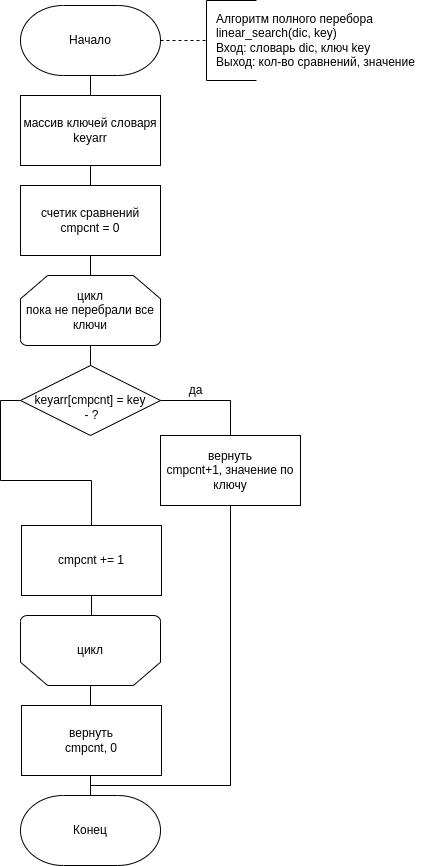
\includegraphics[scale=0.65]{schema_lin.png}}
		\caption*{Рисунок 2.1~--- Алгоритм полного перебора}
	\end{figure}
	
	\begin{figure}[H]
		\center{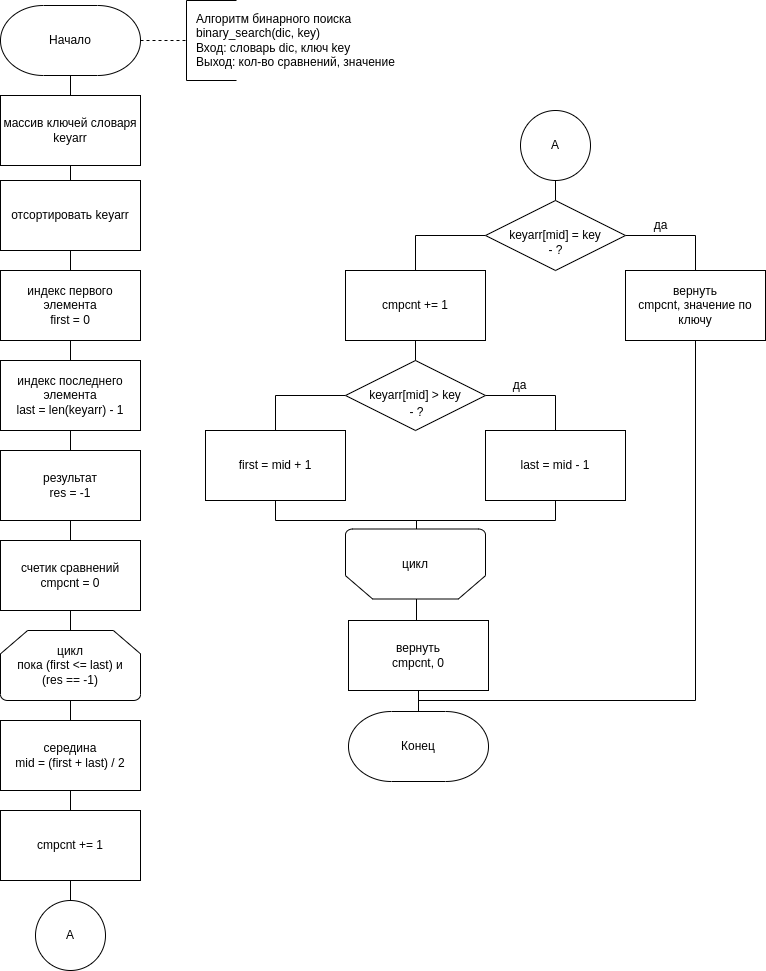
\includegraphics[scale=0.65]{schema_bin.png}}
		\caption*{Рисунок 2.2~--- Бинарный поиск}
	\end{figure}
	
	\begin{figure}[H]
		\center{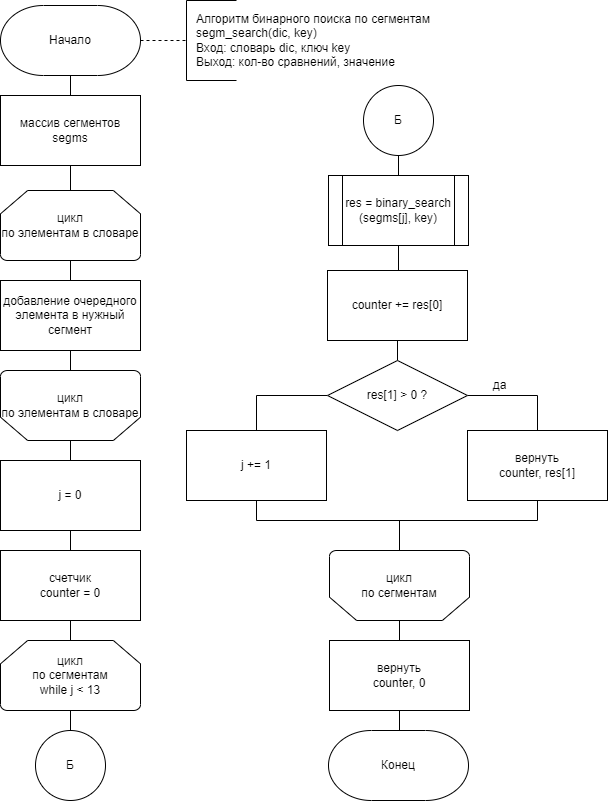
\includegraphics[scale=0.65]{schema_segm.png}}
		\caption*{Рисунок 2.3~--- Бинарный поиск по сегментам}
	\end{figure}
	
	\section*{2.2 Типы и структуры данных}
	\addcontentsline{toc}{section}{2.2 Типы и структуры данных}
	
	Словарь~--- абстрактный тип данных (интерфейс к хранилищу данных), позволяющий хранить пары вида <<ключ : значение>> и поддерживающий
	операции добавления пары, а также поиска и удаления пары по ключу:
	\begin{itemize}
		\item insert(key, value);
		\item get(key);
		\item remove(key).
	\end{itemize}
	В программном обеспечении необходимо использовать встроенный в язык программирования тип данных или реализовать его самостоятельно.
	
	\section*{2.3 Способ тестирования}
	\addcontentsline{toc}{section}{2.3 Способ тестирования}
	
	Создаваемое программное обеспечение будет протестировано методом \verb|черного ящика|. Для тестирования были выделены следующие классы эквивалентности.
	\begin{enumerate}
		\item Неверный выбор режима работы программы~--- пустой ввод, нецифровой символ или вещественное число.
		\item Верный выбор режима работы программы~--- цифра из диапазона $[1..5]$ или целое число, выходящее за пределы указанного диапазона.
	\end{enumerate}
	
	\section*{2.4 Тестовые данные}
	\addcontentsline{toc}{section}{2.4 Тестовые данные}
	
	В таблицах 2.1 -- 2.2 представлены тестовые данные.
	
	\begin{table} [H]
		\caption*{Таблица 2.1~--- Функциональные тесты выбора режима работы программы}
		\begin{tabular}[l]{|c c c|}
			\hline
			Номер тестового случая & Ввод & Ожидаемый результат  \\
			
			1 & \verb|_|\tablefootnote[1]{Пустой ввод} & Неверный ввод \\\hline 
			
			2 & $\alpha$ & Неверный ввод \\\hline
			
			3 & 3.14 & Неверный ввод \\\hline
			
			4 & 1 & Введите ключ для поиска \\\hline 
			
			5 & 2 & Введите ключ для поиска \\\hline
			
			6 & 3 & Введите ключ для поиска \\\hline
			
			7 & 4 & Гистограммы кол-ва сравнений \\\hline
			
			8 & 5 & Выход \\\hline
		\end{tabular}
	\end{table}
	
	\begin{table} [H]
		\caption*{Таблица 2.2~--- Функциональные тесты ввода ключа для поиска}
		\begin{tabular}[l]{|c c c|}
			\hline
			Номер тестового случая & Ввод & Ожидаемый результат  \\
			
			1 & Ключ, которого нет в словаре & 0 вхождений \\\hline
			
			2 & Ключ, который есть в словаре & Число вхождений \\\hline
		\end{tabular}
	\end{table}
	
	\section*{2.5 Структура программного обеспечения}
	\addcontentsline{toc}{section}{2.5 Структура программного обеспечения}
	
	Программное обеспечение разработано с использованием структурного подхода к программированию. Программа содержит функции, отвечающие за поиск ключа в словаре. Функция \verb|linear_search| решает данную задачу методом полного перебора всех возможных ключей. Функция \verb|binary_search| решает задачу с помощью бинарного поиска. Функция \verb|segm_search| решает задачу с помощью бинарного поиска по сегментам. Все три функции принимают на вход словарь и искомый ключ, а возвращают целое число~--- количество сравнений искомого ключа с ключами словаря при поиске и найденное значение по ключу.
	
	\section*{2.6 Вывод по конструкторской части}
	\addcontentsline{toc}{section}{2.6 Вывод по конструкторской части}
	
	В данном разделе были разработаны схемы алгоритмов для поиска ключа в словаре: алгоритма полного перебора, бинарного поиска и бинарного поиска по сегментам, а также подготовлены тестовые данные для программного обеспечения. 
	
	\chapter*{3 Технологическая часть}
	\addcontentsline{toc}{chapter}{3 Технологическая часть}
	
	В данном разделе приведены средства реализации и листинги кода, а также перечислены требования к разрабатываемому программному обеспечению.
	
	\section*{3.1 Требования к ПО}
	\addcontentsline{toc}{section}{3.1 Требования к ПО}
	
	К программе предъявляется ряд требований:
	
	\begin{itemize}
		\item требования ко вводу
		\begin{itemize}
			\item должен быть выбран режим работы программы (целое число в дапазоне $[1..5]$);
			\item должен быть введен искомый ключ (тип данных~--- строка).
		\end{itemize}
		\item требования к выводу
		\begin{itemize}
			\item найден ли искомый ключ в словаре;
			\item какое количество сравнений занял поиск искомого ключа;
			\item гистограммы с указанием зависимости количества сравнений от положения ключа в словаре.
		\end{itemize}
		\item ограничения работы программы
		\begin{itemize}
			\item при вводе режима работы программы, выходящего за пределы указанного диапазона, программа сообщает об ошибке ввода режима работы.
		\end{itemize}
		\item функциональные требования к программному обеспечению
		\begin{itemize}
			\item при запуске программа должна выводить меню с возможными режимами работы;
			\item программа должна осуществлять поиск в словаре с помощью указанных алгоритмов;
			\item в исследовательском режиме программа должна вычислять количества сравнений каждого ключа из словаря при поиске каждым из указанных алгоритмов.
		\end{itemize}
	\end{itemize}
	
	\section*{3.2 Средства реализации}
	\addcontentsline{toc}{section}{3.2 Средства реализации}
	
	Для реализации ПО был выбран язык программирования \verb|Python| [1]. Это обусловлено наличием в нем встроенного типа данных \verb|dict|, который предоставляет необходимый интерфейс для решения задачи, а также знанием возможностей языка.
	
	В качестве среды разработки была выбрана \verb|Visual Studio Code| [3]. Достаточный опыт работы в этой среде, удобства написания кода и его автодополнения стали ключевыми при выборе.
	
	\section*{3.3 Реализация алгоритмов}
	\addcontentsline{toc}{section}{3.3 Реализация алгоритмов}
	
	В листингах 3.1 -- 3.3 приведены реализации алгоритмов, использовавшихся в программном обеспечении.
	
	\begin{lstlisting}[title=Листинг 3.1~--- Алгоритм полного перебора]
		def linear_search(dic : dict, key : str):
		keyarr = list(dic.keys())
		cmpcnt = 0
		while cmpcnt < len(keyarr):
		if keyarr[cmpcnt] == key:
		return cmpcnt + 1, dic.get(key)
		cmpcnt += 1
		return cmpcnt, 0
	\end{lstlisting}
	
	\begin{lstlisting}[title=Листинг 3.2~--- Бинарный поиск]
		def binary_search(dic : dict, key : str):
		keyarr = list(dic.keys())
		keyarr.sort()
		first = 0
		last = len(keyarr)-1
		res = -1
		cmpcnt = 0
		while (first <= last) and (res == -1):
		mid = (first + last) // 2
		cmpcnt += 1
		if keyarr[mid] == key:
		return cmpcnt, dic.get(key)
		else:
		cmpcnt += 1
		if key < keyarr[mid]:
		last = mid - 1
		else:
		first = mid + 1
		return cmpcnt, 0
	\end{lstlisting}
	
	\begin{lstlisting}[title=Листинг 3.3~--- Бинарный поиск по сегментам]
		def segm_search(dic : dict, key : str):
		segms = []
		for i in range(13):
		segms.append(dict())
		for elem in dic:
		value = dic.get(elem)
		if value > 40:
		segms[0].update([(elem, value)])
		elif value > 19:
		segms[1].update([(elem, value)])
		elif value > 10:
		segms[2].update([(elem, value)])
		else:
		for i in range(1, 11):
		if value == i:
		segms[13 - i].update([(elem, value)])
		counter = 0   
		j = 0
		while j < 13:
		res = binary_search(segms[j], key)
		counter += res[0]
		if res[1]:
		return counter, res[1]
		j += 1
		
		return counter, 0
	\end{lstlisting}
	
	\section*{3.4 Пример работы программы}
	\addcontentsline{toc}{section}{3.4 Пример работы программы}
	
	В качестве исходного словаря взята частотная характеристика появления той или иной словоформы в произведении Антона Павловича Чехова <<Человек в футляре>> [2]. Ключом в данном словаре является каждая найденная в тексте словоформа, а значением такого ключа~--- количество употреблений в тексте.
	\newlineНа рисунке 3.1 приведен пример работы программы.
	
	\begin{figure}[H]
		\center{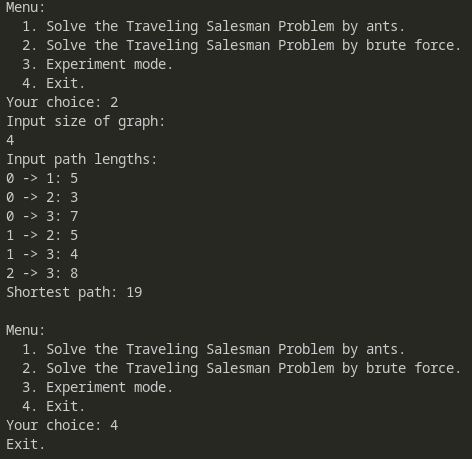
\includegraphics[scale=0.72]{example.PNG}}
		\caption*{Рисунок 3.1~--- Пример работы программы}
	\end{figure}
	
	\section*{3.5 Вывод по технологической части}
	\addcontentsline{toc}{section}{3.5 Вывод по технологической части}
	
	В данном разделе были описаны средства реализации, представлены требования к ПО и реализованы алгоритмы для поиска ключа в словаре: алгоритм полного перебора, бинарного поиска и бинарного поиска по сегментам.
	
	\chapter*{4 Исследовательская часть}
	\addcontentsline{toc}{chapter}{4 Исследовательская часть}
	
	В этом разделе будет исследовано количество сравнений при поиске ключа в словаре с использованием разработанных реализаций алгоритмов.
	
	\section*{4.1 Технические характеристики}
	\addcontentsline{toc}{section}{4.1 Технические характеристики}
	
	Ниже приведены технические характеристики устройства, на котором было проведено тестирование ПО:
	
	\begin{itemize}
		\item операционная система Windows 10 64-разрядная;
		\item оперативная память 16 ГБ;
		\item процессор Intel(R) Core(TM) i5-4690 @ 3.50ГГц.
	\end{itemize}
	
	\section*{4.2 Сравнительный анализ}
	\addcontentsline{toc}{section}{4.2 Сравнительный анализ}
	
	На рисунках 4.1 -- 4.9 представлены зависимости количества сравнений в словаре от позиции ключа при использовании каждого из рассмотренных алгоритмов.
	
	\begin{figure}[H]
		\center{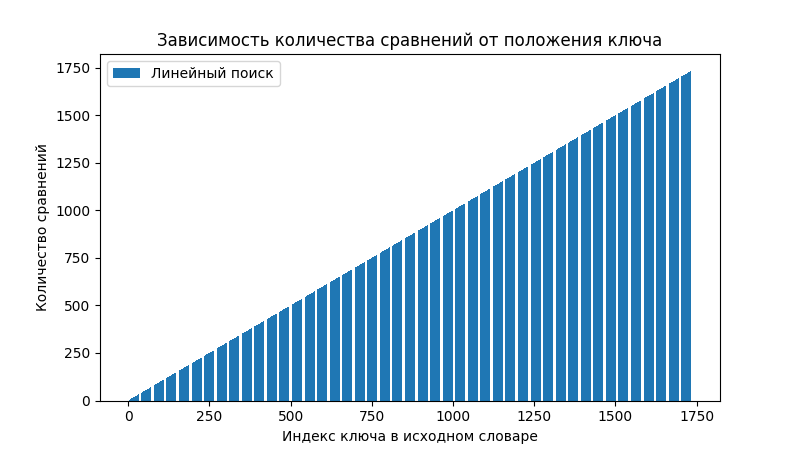
\includegraphics[scale=0.72]{lin1.PNG}}
		\caption*{Рисунок 4.1~--- Зависимость кол-ва сравнений от позиции ключа при полном переборе}
	\end{figure}
	
	\begin{figure}[H]
		\center{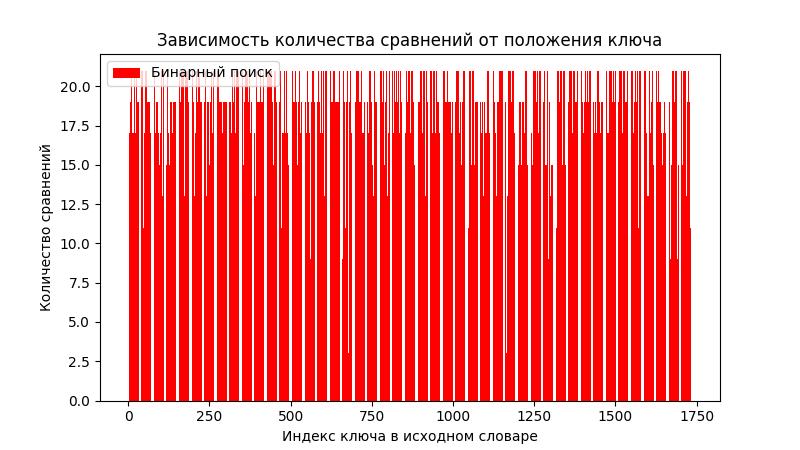
\includegraphics[scale=0.72]{bin1.PNG}}
		\caption*{Рисунок 4.2~--- Зависимость кол-ва сравнений от позиции ключа при бинарном поиске}
	\end{figure}
	
	\begin{figure}[H]
		\center{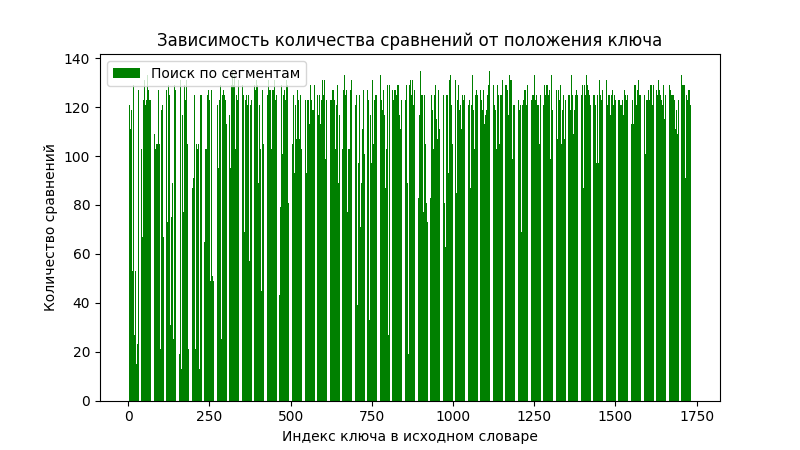
\includegraphics[scale=0.72]{segm1.PNG}}
		\caption*{Рисунок 4.3~--- Зависимость кол-ва сравнений от позиции ключа при бинарном поиске по сегментам}
	\end{figure}
	
	Эти же данные для бинарного поиска и бинарного поиска по сегментам можно упорядочить по убыванию количества сравнений, чтобы увидеть, какие позиции дают наилучшие и наихудшие результаты.
	
	\begin{figure}[H]
		\center{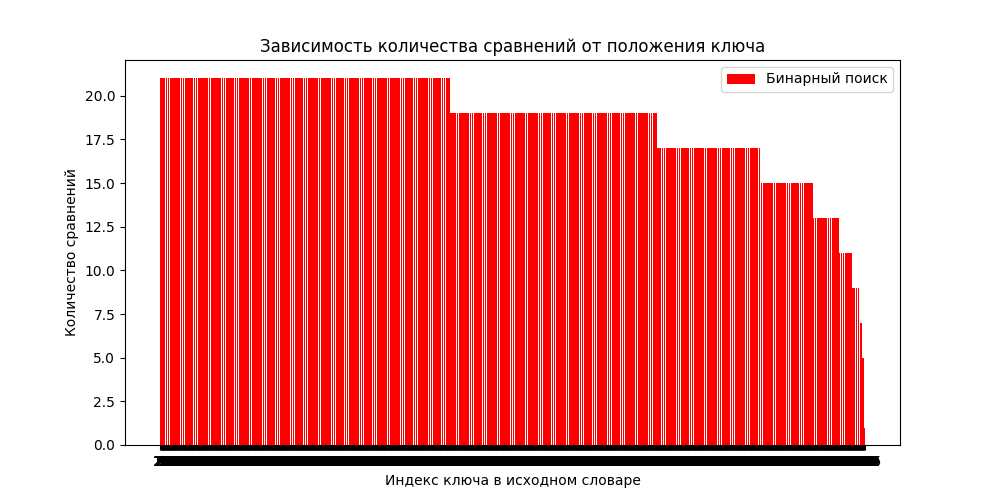
\includegraphics[scale=0.72]{bin2.PNG}}
		\caption*{Рисунок 4.4~--- Зависимость кол-ва сравнений от позиции ключа при бинарном поиске}
	\end{figure}
	
	\begin{figure}[H]
		\center{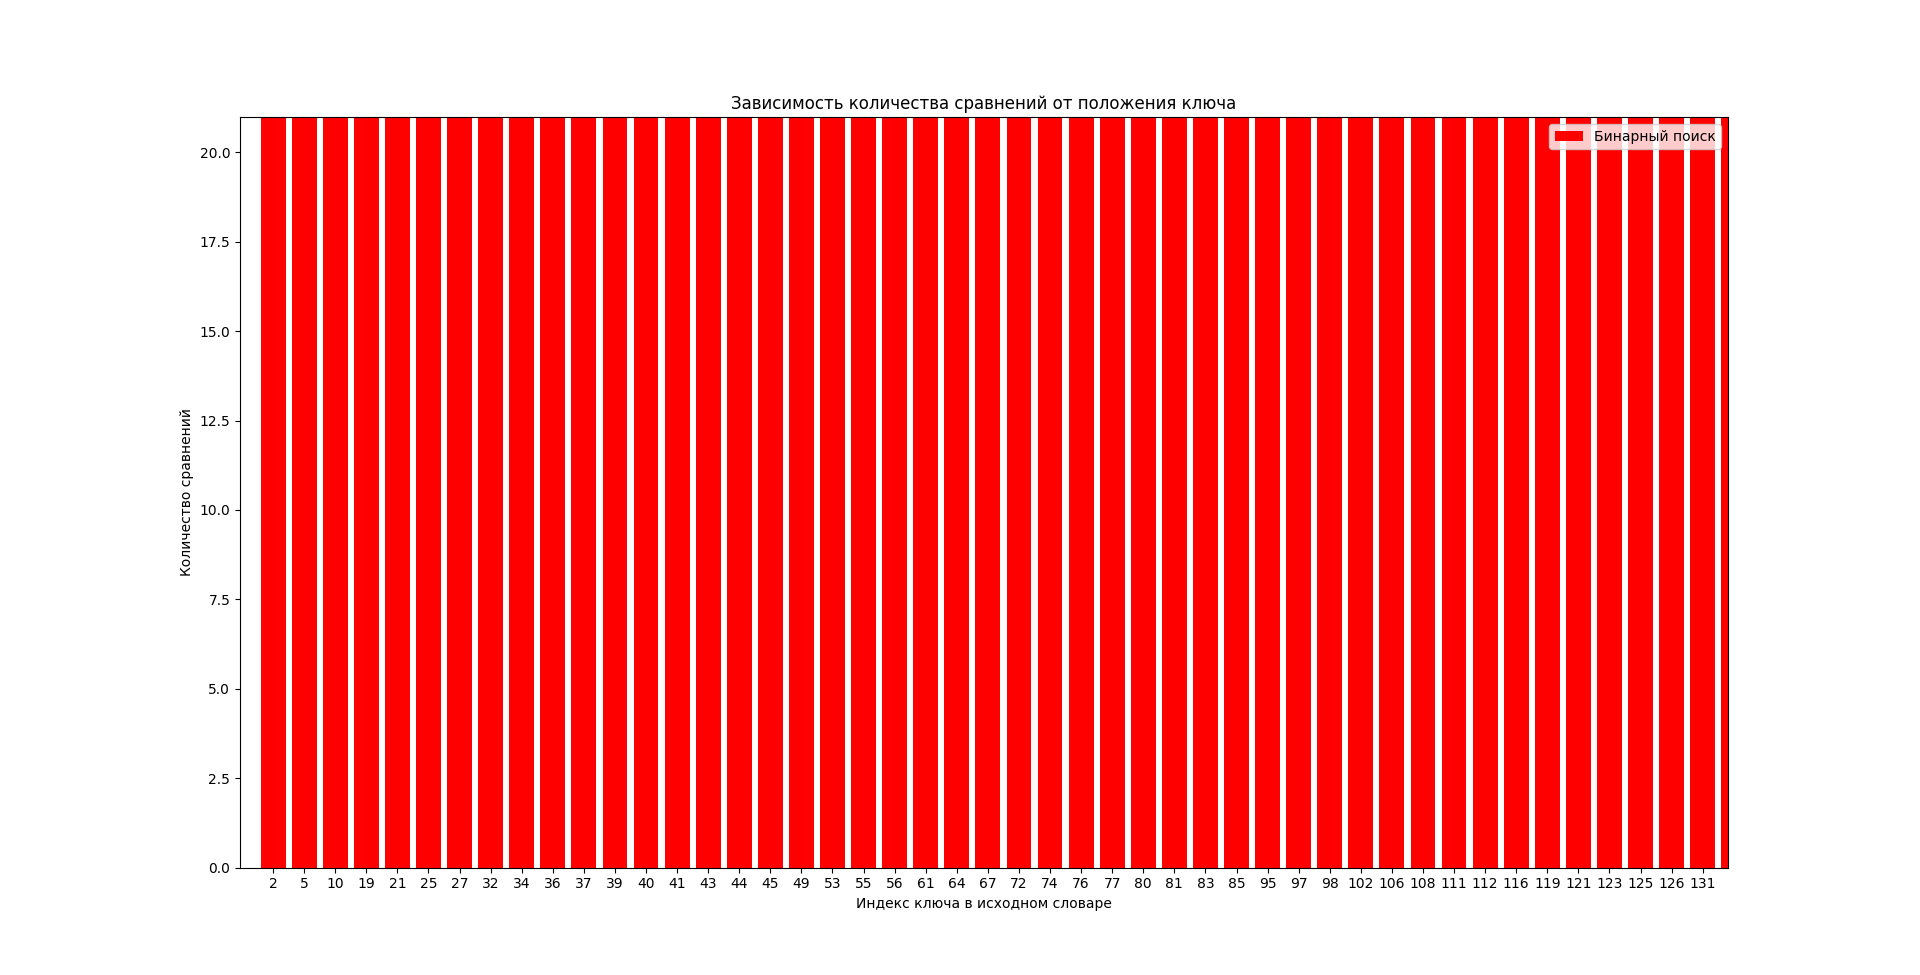
\includegraphics[scale=0.38]{bin2_big.PNG}}
		\caption*{Рисунок 4.5~--- Худший случай при бинарном поиске}
	\end{figure}
	
	\begin{figure}[H]
		\center{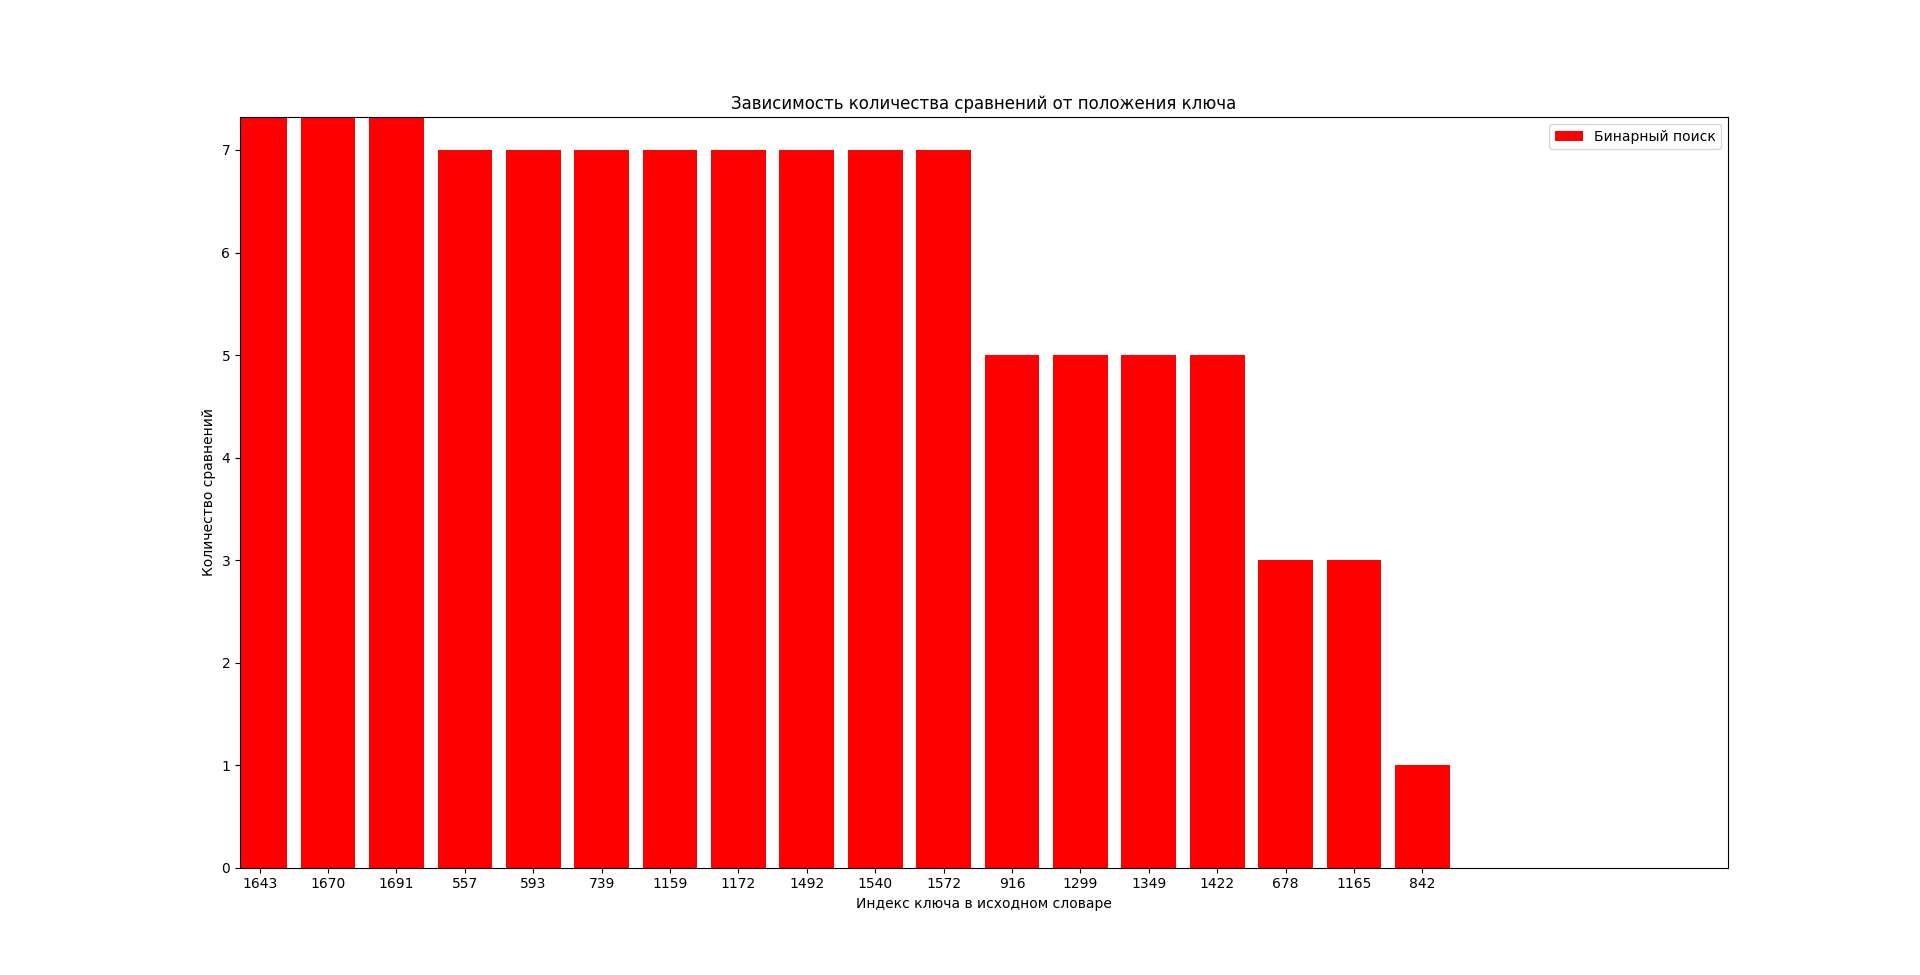
\includegraphics[scale=0.38]{bin2_small.PNG}}
		\caption*{Рисунок 4.6~--- Лучший случай при бинарном поиске}
	\end{figure}
	
	\begin{figure}[H]
		\center{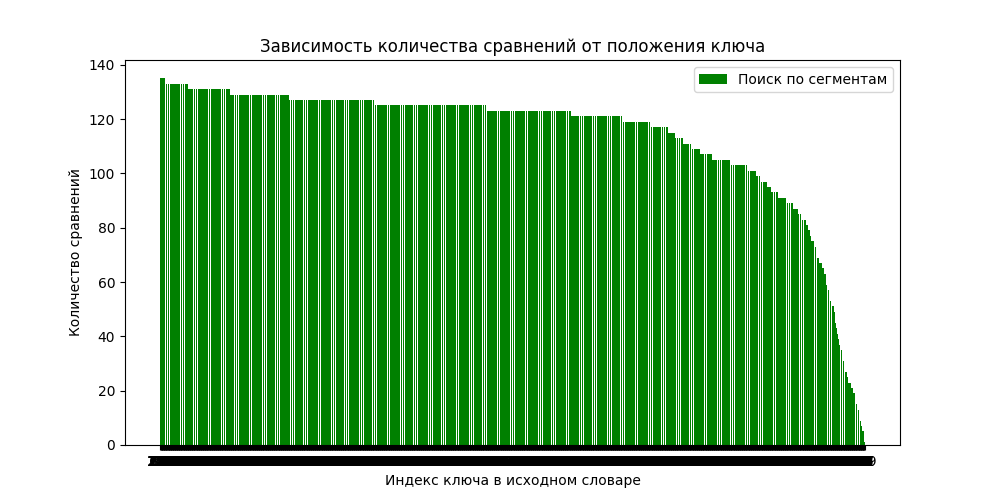
\includegraphics[scale=0.72]{segm2.PNG}}
		\caption*{Рисунок 4.7~--- Зависимость кол-ва сравнений от позиции ключа при бинарном поиске по сегментам}
	\end{figure}
	
	\begin{figure}[H]
		\center{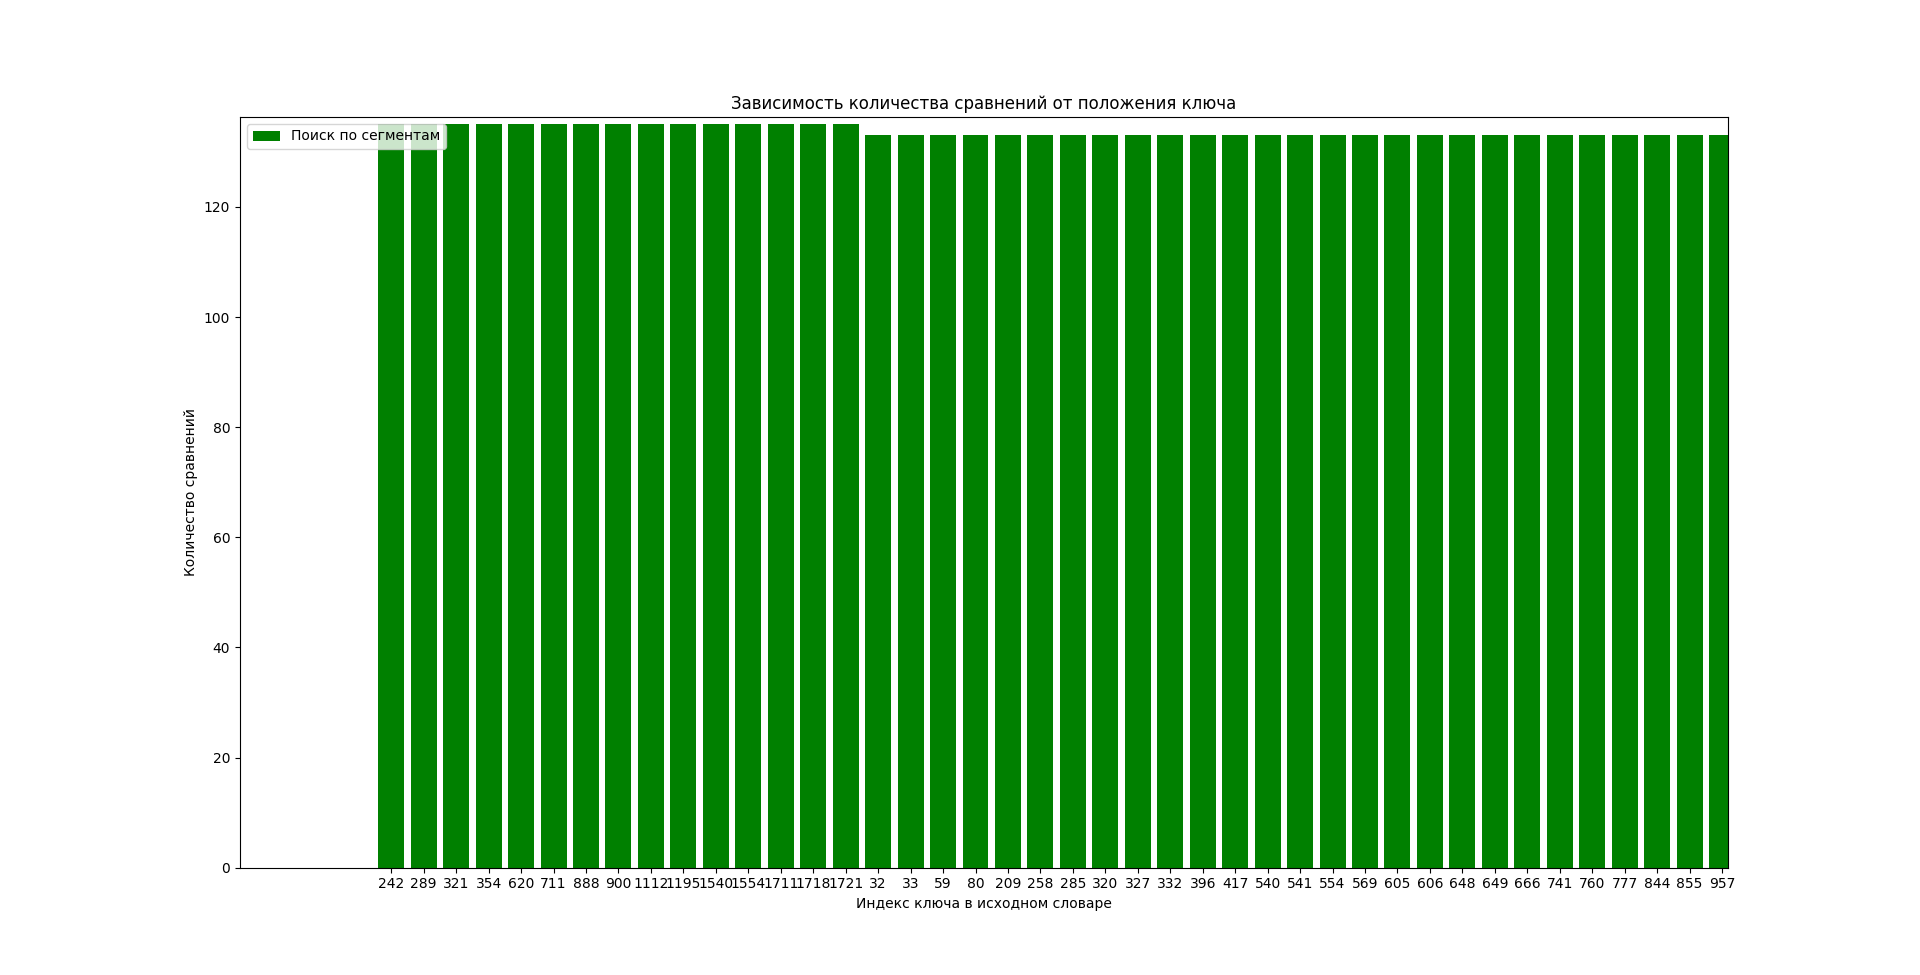
\includegraphics[scale=0.38]{segm2_big.PNG}}
		\caption*{Рисунок 4.8~--- Худший случай при бинарном поиске по сегментам}
	\end{figure}
	
	\begin{figure}[H]
		\center{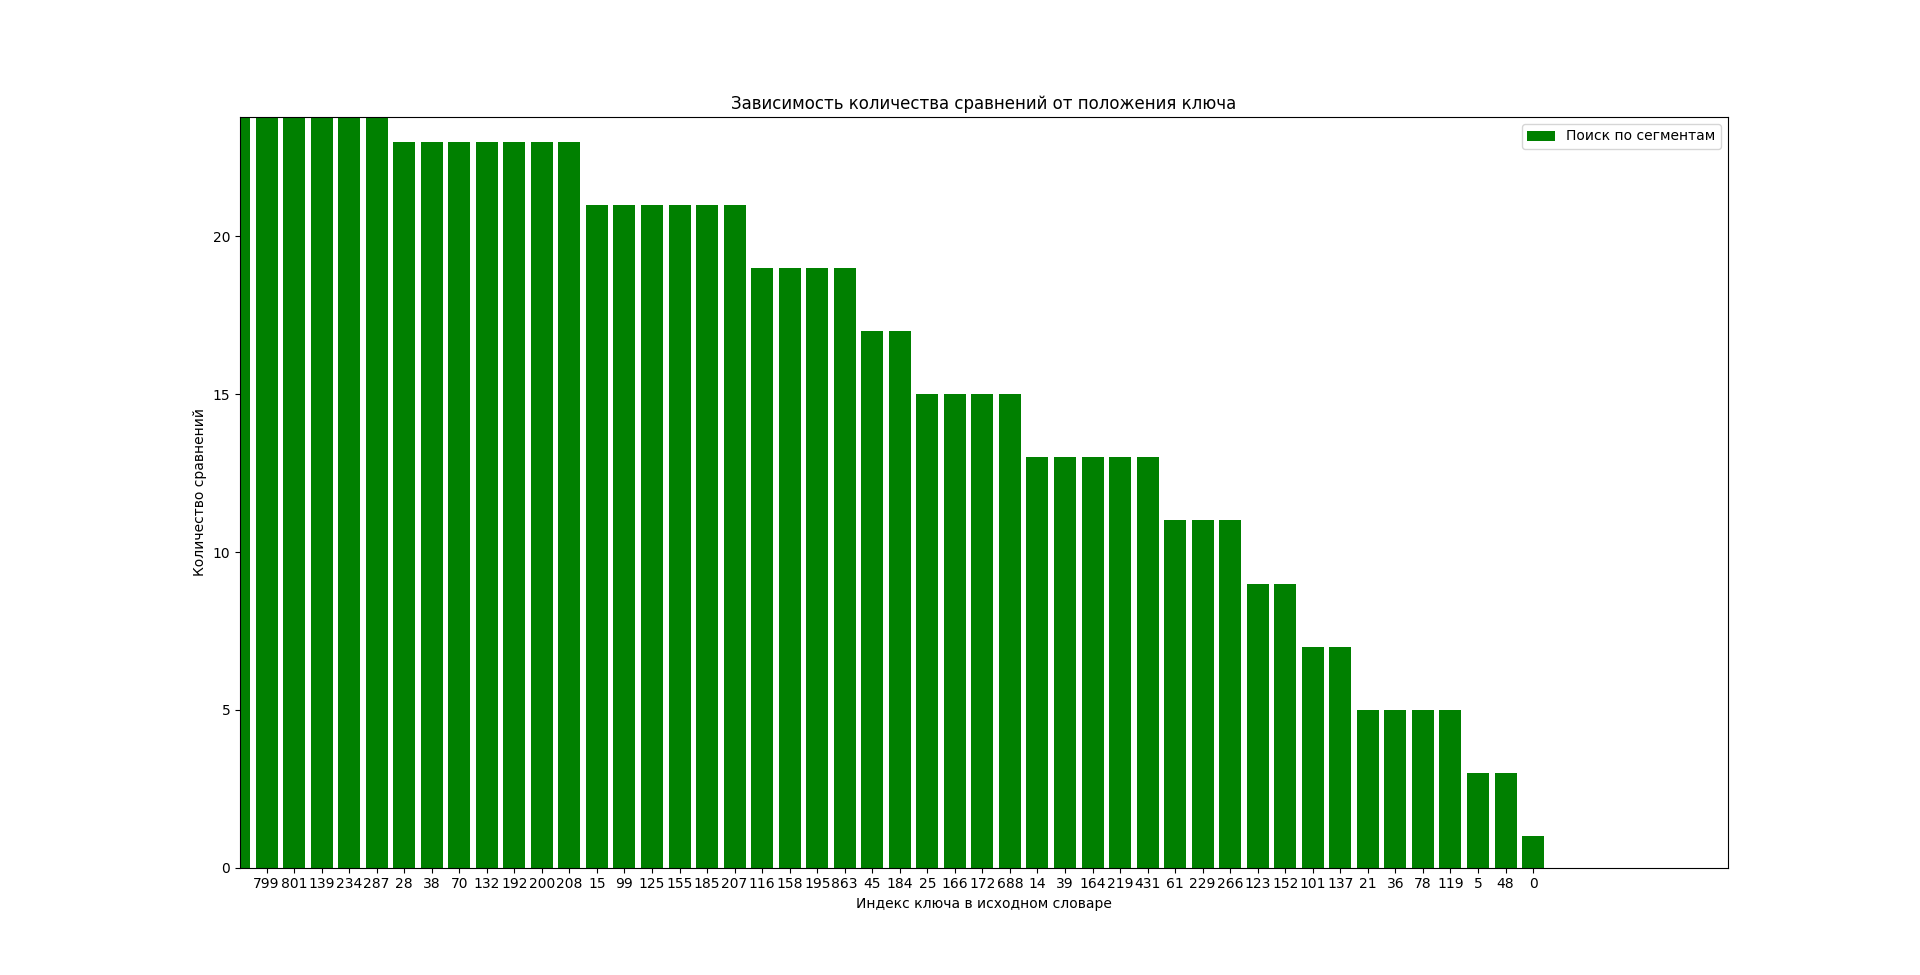
\includegraphics[scale=0.38]{segm2_small.PNG}}
		\caption*{Рисунок 4.9~--- Лучший случай при бинарном поиске по сегментам}
	\end{figure}
	
	\section*{4.3 Вывод по исследовательской части}
	\addcontentsline{toc}{section}{4.3 Вывод по исследовательской части}
	
	По результатам замеров можно сказать, что в среднем бинарный поиск дает наилучший результат, то есть наименьшее количество сравнений при поиске. При выбранном способе сегментирования словаря бинарный поиск по сегментам дает выигрыш только при поиске наиболее часто встречающихся в тексте слов.
	
	В худших случаях алгоритм бинарного поиска также показывает наилучший результат, то есть наименьшее количество сравнений: чуть больше 20, при этом алгоритм бинарного поиска по сегментам сравнивает ключи более 130 раз, что обусловлено выбором способа сегментирования словаря. Алгоритм полного перебора в худшем случае покажет количество ключей в словаре.
	
	В лучшем же случае все три алгоритма показывают одинаковый результат: нахождение искомого ключа за 1 сравнение.
	
	
	\chapter*{Заключение}
	\addcontentsline{toc}{chapter}{Заключение}
	
	В ходе проделанной работы была достигнута поставленная цель и решены следующие задачи:
	
	\begin{itemize}
		\item изучены алгоритмы поиска ключа в словаре: алгоритм полного перебора, бинарного поиска и бинарного поиска по сегментам;
		\item разработаны схемы этих алгоритмов;
		\item реализованы изученные алгоритмы;
		\item проведено тестирование разработанного программного обеспечения;
		\item проведен анализ количества сравнений при поиске в словаре с использованием данных алгоритмов.
	\end{itemize}
	
	Выбор того или иного алгоритма при осуществлении поиска ключа в словаре будет зависеть от исходных данных.
	
	\chapter*{Список литературы}
	\addcontentsline{toc}{chapter}{Список литературы}
	
	[1] Python [Электронный ресурс]. Режим доступа: https://python.org/. Дата обращения: 26.12.2021.\\
	
	[2] Текст произведения А.П. Чехова <<Человек в футляре>> [Электронный ресурс]. Режим доступа: https://ilibrary.ru/text/438/p.1/index.html. Дата обращения: 26.12.2021.\\
	
	[3] Visual Studio Code - Code Editing [Электронный ресурс]. Режим доступа: https://code.visualstudio.com. Дата обращения: 26.12.2021.\\
	
	[4] Алгоритмы поиска [Электронный ресурс]. Режим доступа: \newline https://pythonist.ru/algoritmy-poiska-na-python. Дата обращения: 26.12.2021.
	
\end{document}
